% Copyright 2007 by Till Tantau
%
% This file may be distributed and/or modified
%
% 1. under the LaTeX Project Public License and/or
% 2. under the GNU Public License.
%
% See the file doc/licenses/LICENSE for more details.



\documentclass{beamer}

%
% DO NOT USE THIS FILE AS A TEMPLATE FOR YOUR OWN TALKS�!!
%
% Use a file in the directory solutions instead.
% They are much better suited.
%


% Setup appearance:

\usetheme{Darmstadt}
\usefonttheme[onlylarge]{structurebold}
\setbeamerfont*{frametitle}{size=\normalsize,series=\bfseries}
\setbeamertemplate{navigation symbols}{}


% Standard packages

\usepackage[english]{babel}
\usepackage[latin1]{inputenc}
\usepackage{times}
\usepackage[T1]{fontenc}


% Setup TikZ

\usepackage{tikz}
\usetikzlibrary{arrows}
\tikzstyle{block}=[draw opacity=0.7,line width=1.4cm]


% Author, Title, etc.

\title[Block Partitioning and Perfect Phylogenies] 
{%
  On the Complexity of SNP Block Partitioning Under the Perfect
  Phylogeny Model%
}

\author[Gramm, Hartman, Nierhoff, Sharan, Tantau]
{
  Jens~Gramm\inst{1} \and
  Tzvika~Hartman\inst{2} \and
  Till~Nierhoff\inst{3} \and
  Roded~Sharan\inst{4} \and
  \textcolor{green!50!black}{Till~Tantau}\inst{5}
}

\institute[T�bingen and others]
{
  \inst{1}%
  Universit�t T�bingen, Germany
  \and
  \vskip-2mm
  \inst{2}%
  Bar-Ilan University, Ramat-Gan, Israel
  \and
  \vskip-2mm
  \inst{3}%
  International Computer Science Institute, Berkeley, USA
  \and
  \vskip-2mm
  \inst{4}%
  Tel-Aviv University, Israel
  \and
  \vskip-2mm
  \inst{5}%
  Universit�t zu L�beck, Germany
}

\date[WABI 2006]
{Workshop on Algorithms in Bioinformatics, 2006}



% The main document

\begin{document}

\begin{frame}
  \titlepage
\end{frame}

\begin{frame}{Outline}
  \tableofcontents
\end{frame}


\section{Introduction}

\subsection{The Model and the Problem}

\begin{frame}{What is haplotyping and why is it important?}
  You hopefully know this after the previous three talks\dots
\end{frame}

\begin{frame}[t]{General formalization of haplotyping.}
  \begin{block}{Inputs}
    \begin{itemize}
    \item A \alert{genotype matrix} $G$.
    \item The \alert{rows} of the matrix are \alert{taxa / individuals}.
    \item The \alert{columns} of the matrix are \alert{SNP sites /
        characters}. 
    \end{itemize}
  \end{block}
  \begin{block}{Outputs}
    \begin{itemize}
    \item A \alert{haplotype matrix} $H$.
    \item Pairs of rows in $H$ \alert{explain} the rows of $G$.
    \item The haplotypes in $H$ are \alert{biologically plausible}. 
    \end{itemize}
  \end{block}
\end{frame}


\begin{frame}[t]{Our formalization of haplotyping.}
  \begin{block}{Inputs}
    \begin{itemize}
    \item A genotype matrix $G$.
    \item The rows of the matrix are individuals / taxa.
    \item The columns of the matrix are SNP sites / characters.
    \item<alert@1->
      The problem is directed: one haplotype is known.
    \item<alert@1->
      The input is biallelic: there are only two homozygous
      states (0 and 1) and one heterozygous state (2).
    \end{itemize}
  \end{block}
  \begin{block}{Outputs}
    \begin{itemize}
    \item A haplotype matrix $H$.
    \item Pairs of rows in $H$ explain the rows of $G$.
    \item<alert@1> The haplotypes in $H$ form a perfect phylogeny.
    \end{itemize}
  \end{block}
\end{frame}


\begin{frame}{We can do perfect phylogeny haplotyping efficiently, but
    \dots}
  \begin{enumerate}
  \item \alert{Data may be missing.}
    \begin{itemize}
    \item This makes the problem NP-complete \dots
    \item \dots even for very restricted cases.
    \end{itemize}
    \textcolor{green!50!black}{Solutions:}
    \begin{itemize}
    \item Additional assumption like the rich data hypothesis. 
    \end{itemize}
  \item \alert{No perfect phylogeny is possible.}
    \begin{itemize}
    \item This can be caused by chromosomal crossing-over effects.
    \item This can be caused by incorrect data.
    \item This can be caused by multiple mutations at the same sites.
    \end{itemize}
    \textcolor{green!50!black}{Solutions:}
    \begin{itemize}
    \item Look for phylogenetic networks.
    \item Correct data.
    \item<alert@1->
       Find blocks where a perfect phylogeny is possible.
    \end{itemize}
  \end{enumerate}
\end{frame}


\subsection{The Integrated Approach}

\begin{frame}{How blocks help in perfect phylogeny haplotyping.}
  \begin{enumerate}
  \item Partition the site set into overlapping contiguous blocks.
  \item Compute a perfect phylogeny for each block and combine them.
  \item Use dynamic programming for finding the partition.
  \end{enumerate}

  \begin{tikzpicture}
    \useasboundingbox (0,-1) rectangle (10,2);
    
    \draw[line width=2mm,dash pattern=on 1mm off 1mm]
      (0,1) -- (9.99,1) node[midway,above] {Genotype matrix}
      (0,0.6666) -- (9.99,0.6666)
      (0,0.3333) -- (9.99,0.3333)
      (0,0) -- (9.99,0) node[midway,below] {\only<1>{no perfect phylogeny}};

    \begin{scope}[xshift=-.5mm]
      \only<2->
      {
        \draw[red,block]            (0,.5)   -- (3,.5)
          node[midway,below] {perfect phylogeny};
      }
        
      \only<3->
      {
        \draw[green!50!black,block] (2.5,.5)   -- (7,.5)
          node[pos=0.6,below] {perfect phylogeny};
      }

      \only<4->
      {
        \draw[blue,block]           (6.5,.5) -- (10,.5)
          node[pos=0.6,below] {perfect phylogeny};
      }
    \end{scope}
  \end{tikzpicture}
\end{frame}

\begin{frame}{Objective of the integrated approach.}
  \begin{enumerate}
  \item Partition the site set into \alert{noncontiguous} blocks. 
  \item Compute a perfect phylogeny for each block and combine them. 
  \item<alert@1-> Compute partition while computing perfect
    phylogenies. 
  \end{enumerate}

  \begin{tikzpicture}
    \useasboundingbox (0,-1) rectangle (10,2);

    \draw[line width=2mm,dash pattern=on 1mm off 1mm]
      (0,1) -- (9.99,1) node[midway,above] {Genotype matrix}
      (0,0.6666) -- (9.99,0.6666)
      (0,0.3333) -- (9.99,0.3333)
      (0,0) -- (9.99,0) node[midway,below] {\only<1>{no perfect phylogeny}};

    \only<2->
    {
      \begin{scope}[xshift=-0.5mm]
        \draw[red,block] (0,.5)   -- (3,.5) 
          node[midway,below] {perfect phylogeny}
                         (8,.5) -- (9,.5);

        \draw[green!50!black,block]
          (3,.5)   -- (6,.5)
            node[pos=0.6,below] {perfect phylogeny}
          (6.4,.5)   -- (8,.5)
          (9,.5) -- (10,.5);

        \draw[blue,block] (6,.5) -- (6.4,.5)
          node[midway,below=5mm] {perfect phylogeny};
      \end{scope}
    }
  \end{tikzpicture}
\end{frame}


\begin{frame}{The formal computational problem.}
  We are interested in the computational complexity of \\
  \alert{the function \alert{$\chi_{\operatorname{PP}}$}}:
  \begin{itemize}
  \item It gets genotype matrices as input.
  \item It maps them to a number $k$.
  \item This number is minimal such that the sites can be
    covered by $k$ sets, each admitting a perfect phylogeny.
    \\
    (We call this a \alert{pp-partition}.)
  \end{itemize}
\end{frame}


\section{Bad News: Hardness Results}

\subsection{Hardness of PP-Partitioning of Haplotype Matrices}

\begin{frame}{Finding pp-partitions of haplotype matrices.}
  We start with a special case:
  \begin{itemize}
  \item The inputs $M$ are \alert{already haplotype matrices}.
  \item The inputs $M$ \alert{do not allow a perfect phylogeny}.
  \item What is $\chi_{\operatorname{PP}}(M)$?
  \end{itemize}
  \begin{example}
    \begin{columns}
      \column{.3\textwidth}
      $M\colon$
      \footnotesize
      \begin{tabular}{cccc}
        0 & 0 & 0 & 1 \\
        0 & 1 & 0 & 0 \\
        1 & 0 & 0 & 0 \\
        0 & 1 & 0 & 0 \\
        1 & 0 & 0 & 0 \\
        0 & 1 & 0 & 1 \\
        1 & 1 & 0 & 0 \\
        0 & 0 & 1 & 0 \\
        1 & 0 & 1 & 0
      \end{tabular}%
      \only<2>
      {%
        
\begin{tikzpicture}
          \useasboundingbox (2.9,0);

          \draw [red, opacity=0.7,line width=1cm] (1.7 ,1.9) -- (1.7 ,-1.7);
          \draw [blue,opacity=0.7,line width=5mm] (0.85,1.9) -- (0.85,-1.7)
                                                  (2.55,1.9) -- (2.55,-1.7);
        \end{tikzpicture}
      }
      \column{.6\textwidth}
      \begin{overprint}
        \onslide<1>
        No perfect phylogeny is possible.
        
        \onslide<2>
        \textcolor{blue!70!bg}{Perfect phylogeny}
        
        \textcolor{red!70!bg}{Perfect phylogeny}
        
        $\chi_{\operatorname{PP}}(M) = 2$.
        
      \end{overprint}
    \end{columns}
  \end{example}
\end{frame}

\begin{frame}{Bad news about pp-partitions of haplotype matrices.}
  \begin{theorem}
    Finding \alert{optimal pp-partition of haplotype matrices}\\
    is equivalent to finding \alert{optimal graph colorings}.
  \end{theorem}

  \begin{proof}[Proof sketch for first direction]
    \begin{enumerate}
    \item Let $G$ be a graph.
    \item Build a matrix with a column for each vertex of $G$.
    \item For each edge of $G$ add four rows inducing\\the
      submatrix $\left(
        \begin{smallmatrix}
          0 & 0 \\
          0 & 1 \\
          1 & 0 \\
          1 & 1
        \end{smallmatrix}\right)$.
    \item The submatrix enforces that the columns lie in different
      perfect phylogenies. \qedhere  
    \end{enumerate}
  \end{proof}
\end{frame}

\begin{frame}{Implications for pp-partitions of haplotype matrices.}
  \begin{corollary}
    If $\chi_{\operatorname{PP}}(M) = 2$ for a haplotype matrix $M$,
    we can find an optimal pp-partition in polynomial time. 
  \end{corollary}

  \begin{corollary}
    Computing $\chi_{\operatorname{PP}}$ for haplotype matrices is
    \begin{itemize}
    \item $\operatorname{NP}$-hard,
    \item not fixed-parameter tractable, unless
      $\operatorname{P}=\operatorname{NP}$, 
    \item very hard to approximate.
    \end{itemize}
  \end{corollary}
\end{frame}


\subsection{Hardness of PP-Partitioning of Genotype Matrices}


\begin{frame}{Finding pp-partitions of genotype matrices.}
  Now comes the general case:
  \begin{itemize}
  \item The inputs $M$ are \alert{genotype matrices}.
  \item The inputs $M$ \alert{do not allow a perfect phylogeny}.
  \item What is $\chi_{\operatorname{PP}}(M)$?
  \end{itemize}
  \begin{example}
    \begin{columns}
      \column{.3\textwidth}
      $M\colon$
      \footnotesize
      \begin{tabular}{cccc}
        2 & 2 & 2 & 2 \\
        1 & 0 & 0 & 0 \\
        0 & 0 & 0 & 1 \\
        0 & 0 & 1 & 0 \\
        0 & 2 & 2 & 0 \\
        1 & 1 & 0 & 0 
      \end{tabular}%
      \only<2>
      {%
        
\begin{tikzpicture}
          \useasboundingbox (2.9,0);
          
          \draw [red, opacity=0.7,line width=1cm] (1.7 ,1.3) -- (1.7 ,-1.1);
          \draw [blue,opacity=0.7,line width=5mm] (0.85,1.3) -- (0.85,-1.1)
                                                  (2.55,1.3) -- (2.55,-1.1);
        \end{tikzpicture}
      }
      \column{.6\textwidth}
      \begin{overprint}
        \onslide<1>
        No perfect phylogeny is possible.
        
        \onslide<2>
        \textcolor{blue!70!bg}{Perfect phylogeny}
        
        \textcolor{red!70!bg}{Perfect phylogeny}
        
        $\chi_{\operatorname{PP}}(M) = 2$.
        
      \end{overprint}
    \end{columns}
  \end{example}
\end{frame}


\begin{frame}{Bad news about pp-partitions of haplotype matrices.}
  \begin{theorem}
    Finding \alert{optimal pp-partition of genotype matrices}
    is at least as hard as finding \alert{optimal colorings of
      3-uniform hypergraphs}. 
  \end{theorem}

  \begin{proof}[Proof sketch]
    \begin{enumerate}
    \item Let $G$ be a 3-uniform hypergraph.
    \item Build a matrix with a column for each vertex of $G$.
    \item For each hyperedge of $G$ add four rows inducing\\ the submatrix
      $\left(
        \begin{smallmatrix}
          2 & 2 & 2 \\
          1 & 0 & 0 \\
          0 & 1 & 0 \\
          0 & 0 & 1
        \end{smallmatrix}\right)
      $.
    \item The submatrix enforces that the three columns do not all lie
      in the same perfect phylogeny. \qedhere
    \end{enumerate}
  \end{proof}
\end{frame}

\begin{frame}{Implications for pp-partitions of genotype matrices.}
  \begin{corollary}
    Even if we know $\chi_{\operatorname{PP}}(M) = 2$ for a genotype matrix $M$,\\
    finding a pp-partition of any fixed size is still
    \begin{itemize}
    \item $\operatorname{NP}$-hard,
    \item not fixed-parameter tractable, unless
      $\operatorname{P}=\operatorname{NP}$, 
    \item very hard to approximate.
    \end{itemize}
  \end{corollary}
\end{frame}


\section{Good News: Tractability Results}

\subsection{Perfect Path Phylogenies}

\begin{frame}{Automatic optimal pp-partitioning is hopeless, but\dots}
  \begin{itemize}
  \item The hardness results are \alert{worst-case} results for\\
    \alert{highly artificial inputs}.
  \item \alert{Real biological data} might have special properties
    that make the problem \alert{tractable}.
  \item One such property is that perfect phylogenies are often
    perfect \alert{path} phylogenies:

    In HapMap data, in 70\% of the blocks where a perfect phylogeny
    is possible a perfect path phylogeny is also possible.
  \end{itemize}  
\end{frame}


\begin{frame}{Example of a perfect path phylogeny.}
  \begin{columns}[t]
    \column{.3\textwidth}
    \begin{exampleblock}{Genotype matrix}
      $G\colon$
      \begin{tabular}{ccc}
        A & B & C \\\hline
        2 & 2 & 2 \\
        0 & 2 & 0 \\
        2 & 0 & 0 \\
        0 & 2 & 2 
      \end{tabular}
    \end{exampleblock}

    \column{.3\textwidth}
    \begin{exampleblock}{Haplotype matrix}
      $H\colon$
      \begin{tabular}{ccc}
        A & B & C \\\hline
        1 & 0 & 0 \\
        0 & 1 & 1 \\
        0 & 0 & 0 \\
        0 & 1 & 0 \\
        0 & 0 & 0 \\
        1 & 0 & 0 \\
        0 & 0 & 0 \\
        0 & 1 & 1 
      \end{tabular}
    \end{exampleblock}

    \column{.4\textwidth}
    \begin{exampleblock}{Perfect path phylogeny}
      \begin{center}
        \begin{tikzpicture}[auto,thick]
          \tikzstyle{node}=%
          [%
            minimum size=10pt,%
            inner sep=0pt,%
            outer sep=0pt,%
            ball color=example text.fg,%
            circle%
          ]
        
          \node [node] {} [->]
            child {node [node] {} edge from parent node[swap]{A}}
            child {node [node] {}
              child {node [node] {} edge from parent node{C}}
              edge from parent node{B}
            };
        \end{tikzpicture}
      \end{center}
    \end{exampleblock}
  \end{columns}
\end{frame}


\begin{frame}{The modified formal computational problem.}
  We are interested in the computational complexity of \\
  the function $\chi_{\alert{\operatorname{PPP}}}$:
  \begin{itemize}
  \item It gets genotype matrices as input.
  \item It maps them to a number $k$.
  \item This number is minimal such that the sites can be
    covered by $k$ sets, each admitting a perfect \alert{path} phylogeny.
    \\
    (We call this a ppp-partition.)
  \end{itemize}
\end{frame}



\subsection{Tractability of PPP-Partitioning of Genotype Matrices}

\begin{frame}{Good news about ppp-partitions of genotype matrices.}
  \begin{theorem}
    \alert{Optimal ppp-partitions of genotype matrices} can be
    computed in \alert{polynomial time}. 
  \end{theorem}
  \begin{block}{Algorithm}
    \begin{enumerate}
    \item Build the following partial order:
      \begin{itemize}
      \item Can one column be above the other in a phylogeny?
      \item Can the columns be the two children of the root of a
        perfect path phylogeny?
      \end{itemize}
    \item Cover the partial order with as few compatible chain pairs 
      as possible. 

      For this, a maximal matching in a special graph needs to be
      computed.
    \end{enumerate}
  \end{block}
  \hyperlink{algorithm<1>}{\beamergotobutton{The algorithm in action}}
  \hypertarget{return}{}
\end{frame}

\section*{Summary}

\begin{frame}
  \frametitle<presentation>{Summary}

  \begin{itemize}
  \item
    Finding optimal pp-partitions is \alert{intractable}. 
  \item
    It is even intractable to find a pp-partition when \alert{just two 
      noncontiguous  blocks are known to suffice}.
  \item
    For perfect \alert{path} phylogenies, optimal partitions can be
    computed \alert{in polynomial time}.
  \end{itemize}
\end{frame}


\appendix

\section*{Appendix}

\begin{frame}[label=algorithm]{The algorithm in action.}{Computation of
    the partial order.}
  \begin{columns}[t]
    \column{.4\textwidth}
    \begin{exampleblock}{Genotype matrix}
      $G\colon$
      \begin{tabular}{ccccc}
        A & B & C & D & E \\\hline
        2 & 2 & 2 & 2 & 2 \\
        0 & 1 & 2 & 1 & 0 \\
        1 & 0 & 0 & 1 & 2 \\
        0 & 2 & 2 & 0 & 0
      \end{tabular}
    \end{exampleblock}
    \column{.6\textwidth}
    \begin{exampleblock}{Partial order}
      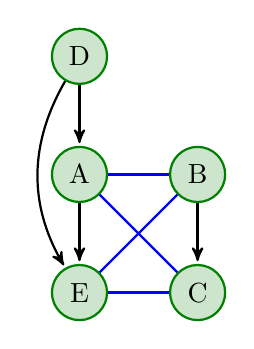
\begin{tikzpicture}[node distance=15mm]
        \tikzstyle{every node}=
        [%
          fill=green!50!black!20,%
          draw=green!50!black,%
          minimum size=7mm,%
          circle,%
          thick%
        ]

        \node (A) {A};
        \node (B) [right of=A] {B};
        \node (C) [below of=B] {C};
        \node (D) [above of=A] {D};
        \node (E) [below of=A] {E};

        \path [thick,shorten >=1pt,-stealth'] (A) edge (E)
                         (B) edge (C)
                         (D) edge (A)
                             edge[bend right] (E);

        \uncover<2>{
        \path [-,blue,thick](A) edge (B)
                                edge (C)  
                            (B) edge (E)
                            (C) edge (E);}
      \end{tikzpicture}

      Partial order: \tikz[baseline] \draw[thick,-stealth'] (0pt,.5ex)
      -- (5mm,.5ex); 

      \uncover<2>{\textcolor{blue}{Compatible as children of root:
          \tikz[baseline] \draw[thick] (0pt,.5ex) -- (5mm,.5ex);}} 
    \end{exampleblock}
  \end{columns}  
\end{frame}

\begin{frame}{The algorithm in action.}{The matching in the special graph.}
  \begin{columns}[t]
    \column{.3\textwidth}
    \begin{exampleblock}{Partial order}
      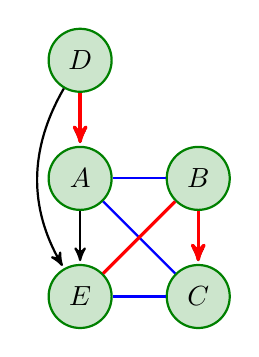
\begin{tikzpicture}[node distance=15mm]
        \tikzstyle{every node}=%
        [%
          fill=green!50!black!20,%
          draw=green!50!black,%
          minimum size=8mm,%
          circle,%
          thick%
        ]

        \node (A)              {$A$};
        \node (B) [right of=A] {$B$};
        \node (C) [below of=B] {$C$};
        \node (D) [above of=A] {$D$};
        \node (E) [below of=A] {$E$};

        \path [thick,shorten >=1pt,-stealth'] (A) edge (E)
                         (B) edge (C)
                         (D) edge (A)
                             edge[bend right] (E);

        \path [-,blue,thick](A) edge (B)
                                edge (C)  
                            (B) edge (E)
                            (C) edge (E);

        \only<3->
        {
          \path[very thick,shorten >=1pt,-stealth',red] (D) edge (A) (B) edge (C);
          \path [-,red,very thick](E) edge (B);
        }
      \end{tikzpicture}
    \end{exampleblock}
    \column{.7\textwidth}
    \begin{exampleblock}{Matching graph}
      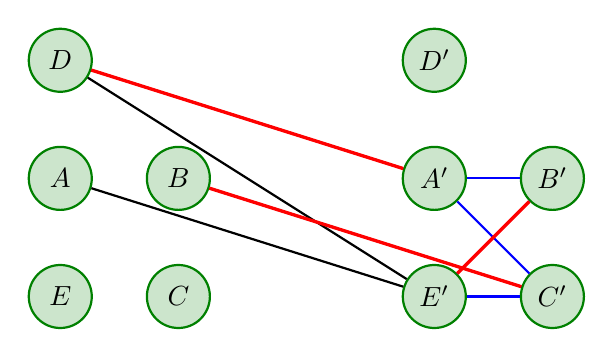
\begin{tikzpicture}[node distance=15mm]
        \tikzstyle{every node}=%
        [%
          fill=green!50!black!20,%
          draw=green!50!black,%
          minimum size=8mm,%
          circle,%
          thick,%
          inner sep=0pt%
        ]

        \node (A)              {$A$};
        \node (B) [right of=A] {$B$};
        \node (C) [below of=B] {$C$};
        \node (D) [above of=A] {$D$};
        \node (E) [below of=A] {$E$};

        \begin{scope}[xshift=4.75cm]
          \node (A')               {$A'$};
          \node (B') [right of=A'] {$B'$};
          \node (C') [below of=B'] {$C'$};
          \node (D') [above of=A'] {$D'$};
          \node (E') [below of=A'] {$E'$};
        \end{scope}
        
        \path [thick]    (A) edge (E')
                         (B) edge (C')
                         (D) edge (A')
                             edge (E');

        \path [blue,thick](A') edge (B')
                               edge (C')  
                          (B') edge (E')
                          (C') edge (E');

        \only<2->
        {
          \path[very thick,red] (D) edge (A')
                           (B) edge (C')
                           (B') edge (E');
        }
      \end{tikzpicture}
    \end{exampleblock}
  \end{columns}

  \medskip
  \uncover<2->{A \alert{maximal matching} in the matching graph
    \uncover<3>{induces\\ \alert{perfect path phylogenies}.}}

  \hfill\hyperlink{return}{\beamerreturnbutton{Return}}
\end{frame}

\end{document}


